\chapter{Off-Chain Design}
\label{chap:offchainDesign}
In this chapter, we present the design of the of-chain components of the \acrlong{ew} environment, which have been developed to offer a user-friendly interface for stakeholders and support the integration of system functionalities. Together with the smart contracts described in \cref{chap:onchainDesign}, these components form the complete system architecture, as illustrated in \cref{fig:fullArchDiag}. 

\begin{figure}[htpb]
  \centering
  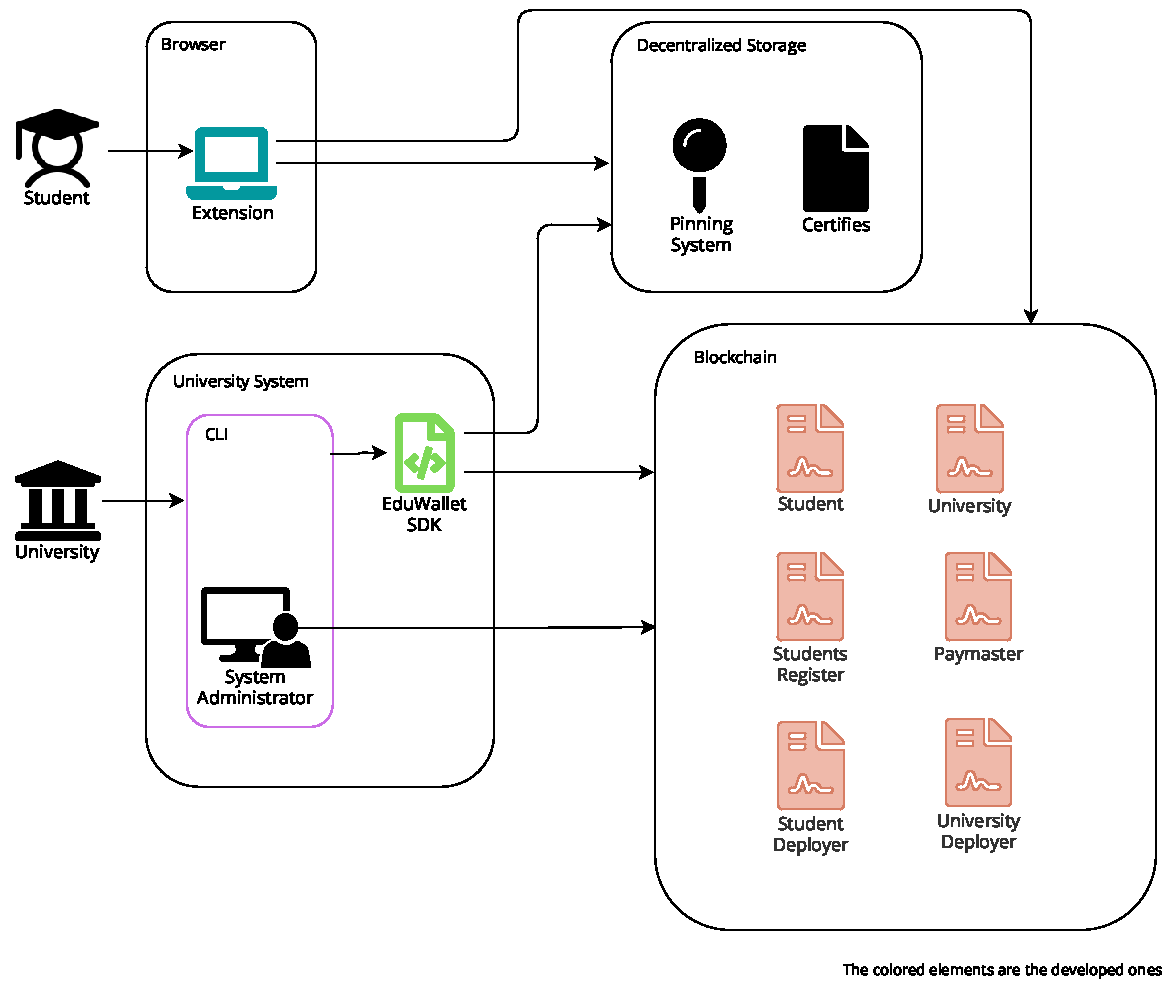
\includegraphics[width=0.8\textwidth]{figures/Architecture diagram complete.pdf}
  \caption[System architecture diagram]{Complete architecture of the \acrlong{ew} system}
  \label{fig:fullArchDiag}
\end{figure}

Given that students using \acrshort{ew} are not expected to have expertise in blockchain technologies, the platform must provide a simple yet effective interface. This interface should enable them to interact with their academic wallets, retrieve academic results, and manage access permissions. These requirements are address \textit{FR 11} in \cref{tab:funcReq}. Similarly, smart contracts interactions may pose challenges even for universities and their \acrfull{it} departments. Therefore, the system must also offer a simplified and accessible interface for institutional use, as specified in \textit{FR 8} in \cref{tab:funcReq}. 
To satisfy these usability needs, two primary components were developed: a \textbf{browser extension} for student interactions with their academic wallets, and a \textbf{\acrlong{sdk}} designed to facilitate the integration of \acrshort{ew} within university systems.

Moreover, \textit{NFR 3} in \cref{tab:nonFuncReq} emphasizes the need to minimize on-chain storage consumption and associated costs by limiting blockchain use to essential data only. To support this goal, the system incorporates a \textbf{decentralized storage} solution, which is responsible for storing and providing access to large data files, such as academic certificates and other supporting documentation.

Finally, to enable comprehensive testing of the environment, a \textbf{\acrlong{cli}} was developed. This tool simulates a real university \acrshort{lms} and allow for testing the \acrshort{sdk} functionalities, as well as its interaction with smart contracts and the decentralized storage layer.

%%%%%%%%%%%%%%%%%%%%%%%%%%%%%%%%%%%%%%%%%%%%%%%%%%%%%%%%%%%%%%%%%%
% BROWSER EXTENSION
%%%%%%%%%%%%%%%%%%%%%%%%%%%%%%%%%%%%%%%%%%%%%%%%%%%%%%%%%%%%%%%%%%

\section{Browser Extension}
\label{sec:browserExtensionDesign}
This section presents the browser extension, which serves as the primary interface for students to interact with their academic wallets. Its main objective is to abstract the complexity of on-chain operations by offering a user-friendly interface that aligns with the design and usability standards of traditional web applications.

\subsection{Technological Choices}
To achieve the highest level of decentralization and autonomy for users, we chose to implement a browser extension rather than a traditional web application. Conventional web applications, typically accessed via a \acrshort{url}, rely on a server to host both the user interface (front-end) and the business logic (back-end), but this architecture introduces central points of control and potential failure. Such reliance would conflict with \textit{NFR 6} in \cref{tab:nonFuncReq}, which emphasizes the importance of minimizing centralization within the system's design.
In contrast, a browser extension operates more like a lightweight desktop application, but within the browser environment. This eliminates the need for an external server to host the interface and, since the core logic of the \acrlong{ew} system resides in smart contracts deployed on the blockchain, no additional server-side back-end is required. This architecture ensures that both the user interface and the underlying logic remain fully decentralized, depending only on the local extension and on-chain infrastructure.
Beyond decentralization, browser extensions offer a compact, wallet-like user experience. Rather than a full screen web page, they present a small, easily accessible window via an icon in the browser toolbar. This interaction model is common among cryptocurrency wallets, such as MetaMask, offering users an intuitive means of managing on-chain assets. Adopting the same paradigm for academic records helps students access and control their data seamlessly, reinforcing the concept on an academic wallet.

Browser extensions are supported across several major browsers, including Microsoft Edge, Google Chrome and Firefox. While each browser introduces minor platform-specific differences, we opted to develop the extension primarily for Google Chrome. Chrome currently holds the largest global browser market share\footnote{\url{https://en.wikipedia.org/wiki/Usage_share_of_web_browsers}}, offering a broad potential user base. Additionally, since Google Chrome and Microsoft Edge are both based on the Chromium open-source project, extensions developed for Chrome are also compatible with Microsoft Edge, further extending platform reach without additional development overhead.

Among the various technologies available for browser extension development, we selected TypeScript as the core programming language and \textit{React} as the framework for building the user interface. TypeScript offers the flexibility and web-centric capabilities of JavaScript while introducing static typing, which improves code safety, clarity and maintainability. It also integrates seamlessly with smart contract development, as libraries exist to generate TypeScript types directly from contract definitions (see CONTRACT\_IMPLEMENTATION\_SECTION).
React, originally developed by Facebook as an open-source JavaScript library, is widely used for building modern web interfaces. It enables efficient \acrshort{ui} development and facilitates seamless interaction with application logic.
Our familiarity and prior experience with both React and JavaScript also influenced our choice, enabling a faster and more reliable development process. Additionally we employed \textit{Vite} as the building tool for our environment, making it easier to manage and bundle the various modules of our browser extension efficiently.

\section{Software Development Kit}
\label{sec:sdkDesign}

\section{Decentralized Storage System}
\label{sec:decStorageDesgn}
This section presents our solution to one of the most significant challenges in blockchain-based systems: the high cost of on-chain storage. To address this issue, presented also through the \textit{NFR 3} in \cref{tab:nonFuncReq}, we introduce an off-chain decentralized storage solution in our project. This system is used to store and retrieve certification files, such as language certificates or graduation diplomas, which require significantly more space than plain text\footnote{PDF files typically range from a few kilobytes to several megabytes, whereas plain text data usually occupies only a few bytes.}. Storing such documents directly on-chain would result in substantial gas costs, making the approach impractical. 

We chose a decentralized storage system over traditional local or cloud-based solutions to maintain the decentralized nature of our environment and to meet \textit{NFR 6} outlined in \cref{tab:nonFuncReq}. Among the various decentralized options available, we selected \acrfull{ipfs} for its ability to provide verifiable and distributed file storage. This choice is motivated by several factors: \acrshort{ipfs} is an open source protocol with a large and active community, strong support, and widespread adoption. It also serves as the foundational layer for many other decentralized platforms, such as Filecoin\footnote{\url{https://filecoin.io}} and Web3.Storage\footnote{\url{https://web3.storage}}, allowing future extensions or upgrades to be implemented with minimal effort \cite{erikflorian2022ipfsandfrineds}. Furthermore, \acrshort{ipfs} ensures immutability of stored files, a critical feature for academic certificates, which must remain unchanged over time.

\subsection{Pinning files}
To fully leverage \acrshort{ipfs}, we integrated Filebase\footnote{\url{https://filebase.com}}, a third-party pinning service. Pinning refers to the act of instructing a node to keep a copy of a file permanently, preventing it from being removed during garbage collection. Without Filebase, we would have needed to run our own local \acrshort{ipfs} node and manage file pinning manually, an approach that introduces instead complexity, higher maintenance costs, and reduced data availability in a testing system like ours. In contrast, Filebase handles node operation and file pinning, offering an accessible solution thorough its AWS S3-compatible \acrshort{api}, which simplifies file uploads to the peer-to-peer network. Notably, Filebase also provides a free tier allowing up to 5 GB of storage, which is sufficient for our needs. This is an advantage over other pinning solutions such as Web3.Storage, which lacks a fully free plan, or Pinata\footnote{\url{https://pinata.cloud}}, which offers more limited options.

\subsection{Integration in the system}
As shown in \cref{fig:fullArchDiag}, both the browser extension and the \acrshort{sdk} interact with the storage system. The browser extension retrieves certificate associated with academic records using the official \acrshort{ipfs} public gateway. It presents students with a direct link to each certificate, composed by the gateway's base \acrshort{url} followed by the file's \acrfull{cid} on the \acrshort{ipfs} network. The \acrshort{cid} of each document is stored on-chain within the student's academic wallet, alongside other record information such as the course name (see \cref{sec:studentContract}). This enables students to view and download their certificates from a standard web interface.

% TODO: Add photo of the extension where you can see the link of a certification
Similarly, the \acrshort{sdk} uses the same mechanism to retrieve certificates on behalf of universities. When uploading a file, however, the \acrshort{sdk} interacts directly with Filebase to ensure the file is pinned and hosted by an active node. The \acrshort{sdk} receives the document from the university, then uses the AWS S3-compatible \acrshort{api} to upload it. The \acrshort{api} requires the key associated with the pinning account (managed by the \acrshort{ew} system administrator) and the file itself. In return, it provides the \acrshort{cid}, which is then stored in the academic record.
% TODO: Reference implementation section

\subsection{Security and Limitations}
Academic certifies, and official documents more broadly, are legal artifacts that must always be secure and verifiable. \acrshort{ipfs} inherently supports these properties through its use of content-based addressing. In this model, each file is identified by a \acrshort{cid}, which is derived from the cryptographic hash of the file's content. Any alteration to the file results in a completely different \acrshort{cid}, ensuring that tampering is immediately detectable \cite{benet2014ipfscontentaddressed}. Since the \acrshort{cid} is stored on the blockchain at the time the certificate is issued by the university, the document's authenticity and integrity are guaranteed.

While \acrshort{ipfs} offers strong immutability and verifiability, it lacks built-in access control. In the context of our system, we assume that certificates are publicly accessible documents. Consequently, any part in possession of a file's \acrshort{cid} can retrieve it via the public gateway. However, if access control becomes a requirement, there are several strategies to address this limitation \cite{barbaraanrealaura2021datapersistence}. One option is to encrypt files before uploading them to \acrshort{ipfs}, such that only authorized components within our system can decrypt them. Another approach is to use a private \acrshort{ipfs} network, where access can be restricted to approved entities. The trade-offs and potential implications of such private deployment will be discussed in the FUTURE\_WORK\_REFERENCE.

\section{CLI}
\label{sec:cliDesign}
This section describes the testing tool developed to evaluate the use of the \acrshort{sdk}. In a real-world deployment, universities are expected to integrate the \acrshort{sdk} into their existing \acrshort{lms} to interact with \acrlong{ew}. However, given that this is a testing environment, smaller and simpler than a real-world deployment, we developed a minimal \acrlong{cli} to simulate the interaction between a university's system and our academic register. We opted to implement a CLI rather than a web application or desktop GUI and this decision allowed for faster development, enabling us to focus on the core functionalities of the \acrshort{sdk}, the blockchain logic, and the browser extension, without introducing additional complexity related to graphical or \acrfull{ux} design.

\cref{fig:clifigs} illustrates the visual aspects of the \acrshort{cli}. In \cref{sfig:cliDesign1}, users can navigate through a sliding menu offering various options. When input is required, the interface prompts the user for the necessary information and provides visual feedback upon completion of the operation (\cref{sfig:cliDesign2}).The \acrshort{cli} leverages the \textit{inquirer}\footnote{\url{https://www.npmjs.com/package/inquirer}} TypeScript library to manage user interactions and uses \textit{ora}\footnote{\url{https://www.npmjs.com/package/ora}} to display feedback. Specifically, \textit{ora} is responsible for showing success and error messages, as well as animated text with spinners to indicate ongoing operations.

\begin{figure}
    \centering
    \begin{subfigure}{.5\textwidth}
        \centering
        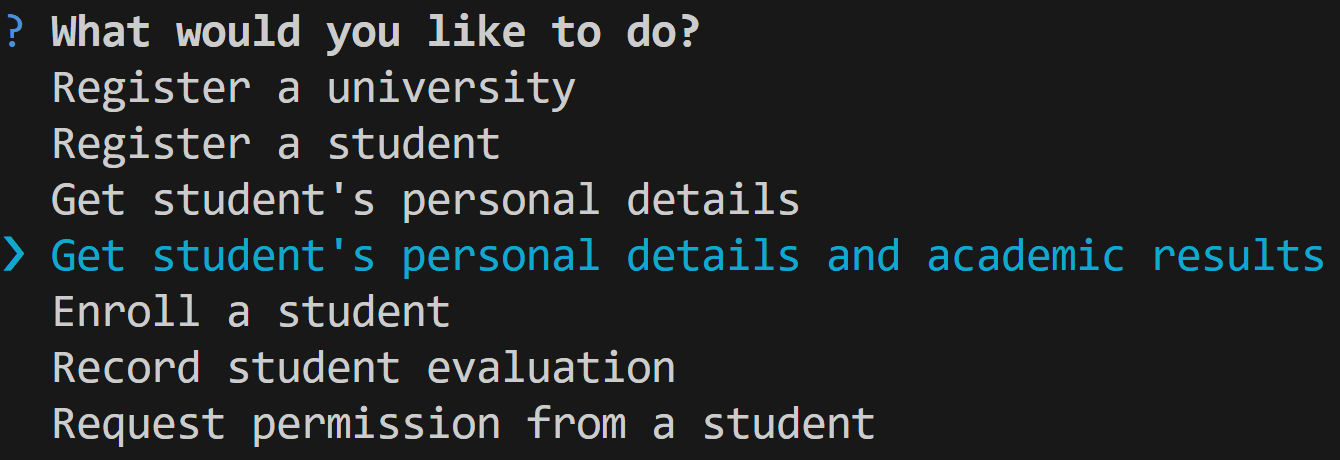
\includegraphics[width=\textwidth]{figures/CLI screen 1.png}
        \caption{Sliding menu}
        \label{sfig:cliDesign1}
    \end{subfigure}
    \hfill
    \begin{subfigure}{.60\textwidth}
        \centering
        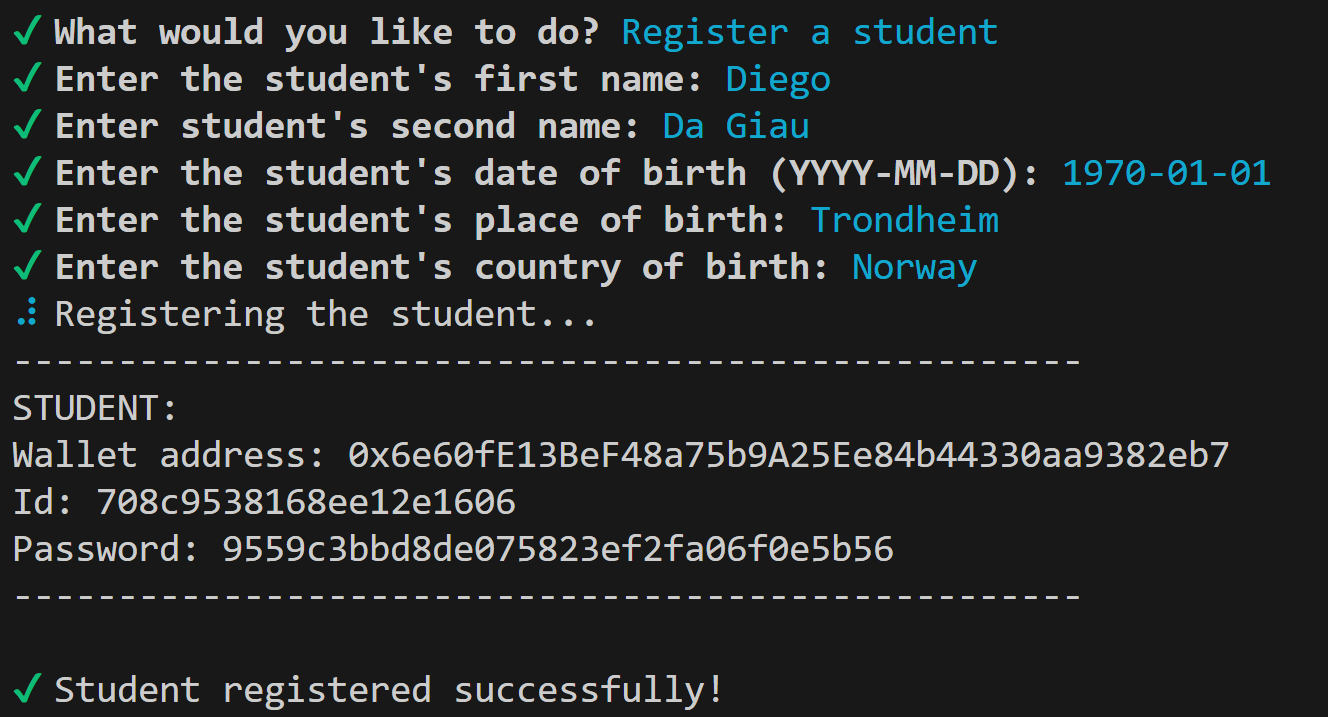
\includegraphics[width=\textwidth]{figures/CLI screen 2.png}
        \caption{User input and visual feedbacks}
        \label{sfig:cliDesign2}
    \end{subfigure}
    \caption[Different aspects of the \acrshort{cli} interface.]{Snapshots of the \acrshort{cli} interface}
    \label{fig:clifigs}
\end{figure}

\subsection{Functionalities}
The \acrshort{cli} exposes all the functionalities outlined in \cref{fig:useCaseCli}. Users can:
\begin{itemize}
    \item Submit a request to register a university in the \acrshort{ew} system.
    \item Register a new student.
    \item Retrieve a student’s personal details.
    \item Retrieve a student’s details and academic results.
    \item Enrol a student in a new course.
    \item Evaluate a student.
    \item Request permissions from a student.
    \item Verify existing permissions.
\end{itemize}
Additionally, the \acrshort{cli} provides options to change the current university and exit the program.

\begin{figure}
  \centering
  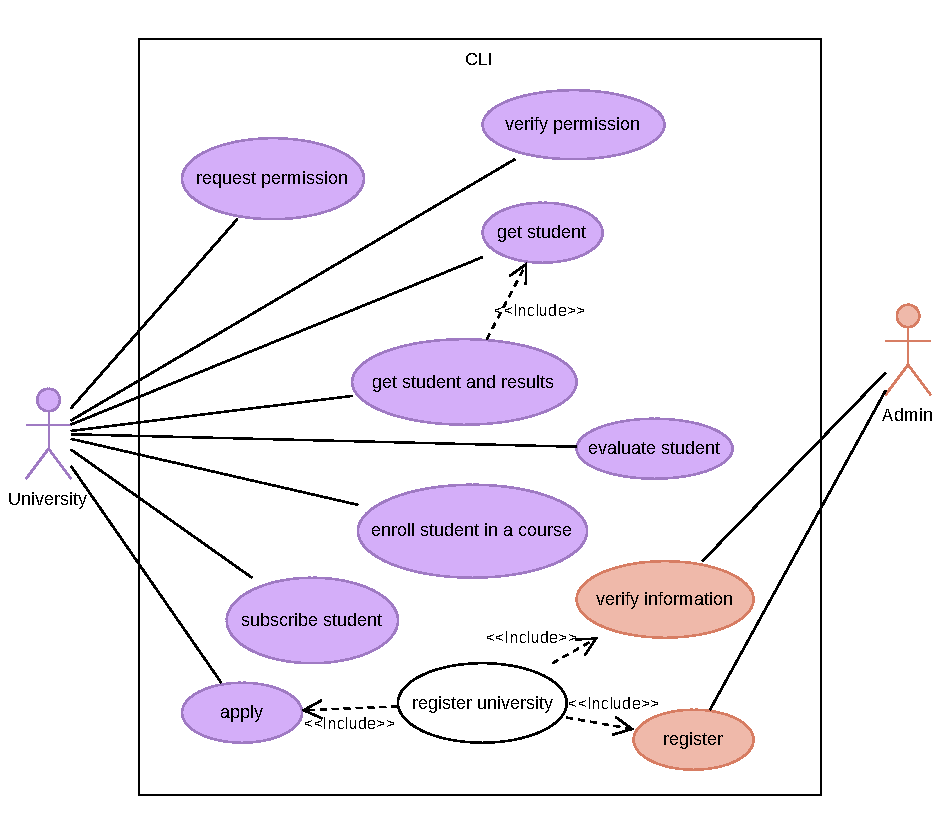
\includegraphics[width=0.8\textwidth]{figures/CLI use case diagram.pdf}
  \caption[\acrshort{cli} use case diagram]{Use case diagram representing the functionalities provided by the \acrshort{cli}.}
  \label{fig:useCaseCli}
\end{figure}

\subsubsection{Testing environment initialization}
Before performing any operation, the \acrshort{cli} must initialize a local blockchain test network by deploying the following smart contracts:
\begin{itemize}
    \item EntryPoint
    \item StudentDeployer
    \item UniversityDeployer
    \item Paymaster
    \item StudentsRegister
\end{itemize}
The \textit{Paymaster} contract then must also be funded to sponsor users' transactions.

In public testnets or in production networks, this initialization step would be unnecessary, as the contracts would already be deployed. Their addresses would be hardcoded in the \acrshort{cli}, \acrshort{sdk} and browser extension.

\subsubsection{University registration}
\label{sssec:applyEw}
To apply to the \acrshort{ew} system, a university must provide its name, country, and short name. Upon completion, it receives the private key of the wallet that owns its smart account. This key is used by the \acrshort{cli} to generate the university's \acrlong{eth} wallet, which is then stored as the current active university. In a real \acrshort{lms}, the private key must be securely stored and used to initialize the wallet and use the \acrshort{sdk}. 

To interact with the EntryPoint  contract in the local testnet, the \acrshort{cli} also funds the university's \acrshort{eth} wallet. In public or production networks, this is not necessary, as the bundler pays the transaction fees and is reimbursed by the Paymaster .

\subsubsection{Register a new student}
To register a student, the  university provides their name, surname, date of birth, place of birth and country of birth. The \acrshort{cli} then calls the \acrshort{sdk} to create the student's academic wallet and credentials, which are returned to the university (\cref{sfig:cliDesign2}). The academic wallet address uniquely identifies the student and must be stored by the university, as it is required for all future interactions. 

The \acrshort{cli} also funds the student's \acrlong{eth} wallet  for local testing. The wallet address is obtained from the login credentials, as explained  for the browser extension in \cref{sec:browserExtensionDesign}.

\subsubsection{Student Information Retrieval}
To retrieve a student's personal information or full academic record, university must provide the student's academic wallet address. The \acrshort{cli} then returns the requested data.

\subsubsection{Enrol and evaluate}
To enrol or evaluate a student, the university must provide the academic wallet address and course code. Enrolment also requires the course name, number of \acrshort{ects} and degree course name (e.g., \textit{Master's in Computer Engineering}, or \textit{Bachelor's in Biology}). Evaluation requires the evaluation date and, optionally, the path to a certificate file. Since the \acrshort{sdk} allows enrolment in or evaluation of multiple courses at once, the \acrshort{cli} also supports submitting multiple records in a single command.     

\subsubsection{Permissions: Request and Verification}
To access or modify student's academic records, the university must request permission. The \acrshort{cli} requires the student's wallet address and the type of permission (read or write). As in most systems, write permission implies read access.
The \acrshort{cli} also includes an option to verify whether the university currently has read or write permission for a specific student.

\subsubsection{Changing University and Exiting the \acrshort{cli}}
These functionalities are unique to the \acrshort{cli} and are included for convenience. To change the active university, the user provides the private key of another registered university. To exit the \acrshort{cli}, the user selects the corresponding menu option.

\subsubsection{Administrator Functionalities}
The \acrshort{cli} also includes admin functionalities, as outlined  in \textit{FR 1} of \cref{tab:funcReq}, to facilitate system testing. Specifically, the administrator can:
\begin{itemize}
    \item Review the information submitted in university registration request.
    \item Approve and register universities in the system.
\end{itemize}
These functionalities are embedded within the university registration option. A university is automatically registered when its information is provided by the user during the registration process.

\subsection{Data validation}
All user input is validated using regular expressions and formatting rules. For instance, wallet addresses and private keys are validated based on length and structure\footnote{Private keys must start with \textit{0x} and be followed by 64 hexadecimal characters; addresses by 42.}. Strings are validated to fall within predefined length limits. Dates must follow the \textit{YYYY-MM-DD} format to avoid ambiguity and must be after January 1, 1970, as they are stored as Unix timestamps (unsigned integers). \acrshort{ects} values are checked to ensure they are valid integers or floating-point numbers within acceptable limits. Since the smart contracts store \acrshort{ects} as integers scaled by 100 (see \cref{sec:studentContract} for further details), the \acrshort{cli} ensures the values will not cause overflow during storage.